\documentclass[11pt,a4paper]{article}

% ─── Packages ────────────────────────────────────────────────────────────────
\usepackage[a4paper, top=2.2cm, bottom=2.2cm, left=2.5cm, right=2.5cm]{geometry}
\usepackage[T1]{fontenc}
\usepackage[utf8]{inputenc}
\usepackage{lmodern}
\usepackage{microtype}
\usepackage{xcolor}
\usepackage{colortbl}
\usepackage{titlesec}
\usepackage{fancyhdr}
\usepackage{graphicx}
\usepackage{booktabs}
\usepackage{tabularx}
\usepackage{array}
\usepackage{longtable}
\usepackage{listings}
\usepackage{enumitem}
\usepackage{tikz}
\usepackage{mdframed}
\usepackage{tcolorbox}
\usepackage{amsmath}
\usepackage{hyperref}
\usepackage{parskip}
\usepackage{setspace}
\usepackage{caption}
\usepackage{float}
\usepackage{pifont}
\usepackage{soul}

\usetikzlibrary{shapes.geometric, arrows.meta, positioning, fit, backgrounds,
                decorations.pathmorphing, shadows, calc}

\tcbuselibrary{breakable, skins}

% ─── Colour Palette ───────────────────────────────────────────────────────────
\definecolor{PrimaryBlue}{HTML}{1A237E}
\definecolor{DeepNavy}{HTML}{0D1B5E}
\definecolor{AccentCyan}{HTML}{00B4D8}
\definecolor{AccentTeal}{HTML}{0096C7}
\definecolor{AccentOrange}{HTML}{F57C00}
\definecolor{AccentGold}{HTML}{FFB300}
\definecolor{LightBg}{HTML}{E8EEF9}
\definecolor{DarkGray}{HTML}{263238}
\definecolor{MidGray}{HTML}{546E7A}
\definecolor{SoftGray}{HTML}{ECEFF1}
\definecolor{RowAlt}{HTML}{F0F4FF}
\definecolor{SuccessGreen}{HTML}{1B5E20}
\definecolor{CodeBg}{HTML}{1E2B3A}
\definecolor{CodeFg}{HTML}{CDD9E5}
\definecolor{RuleLine}{HTML}{1A237E}
\definecolor{MongoGreen}{HTML}{1B5E20}
\definecolor{HiveYellow}{HTML}{E65100}
\definecolor{PigPink}{HTML}{880E4F}
\definecolor{MRBlue}{HTML}{0D47A1}

% ─── Hyperref ─────────────────────────────────────────────────────────────────
\hypersetup{
  colorlinks=true,
  linkcolor=AccentTeal,
  urlcolor=AccentCyan,
  citecolor=AccentOrange,
  pdftitle={Phase 1 Report - Multi-Pipeline ETL Framework},
  pdfauthor={DAS 839 Group}
}

% ─── Section Styling ──────────────────────────────────────────────────────────
\titleformat{\section}{
  \large\bfseries\color{PrimaryBlue}
}{%
  \hspace{-2pt}%
  \tikz[baseline=-0.5ex]\fill[AccentCyan] (0,0) rectangle (4pt,1.1em);%
  \hspace{6pt}%
  \colorbox{PrimaryBlue}{\textcolor{white}{\quad\thesection\quad}}%
}{0.7em}{}[{\color{AccentCyan}\titlerule[1.5pt]}]

\titleformat{\subsection}{
  \normalsize\bfseries\color{DarkGray}
}{%
  \tikz[baseline=-0.4ex]\fill[AccentCyan!60] (0,0) rectangle (3pt,0.9em);%
  \hspace{5pt}\thesubsection%
}{0.6em}{}[{\color{AccentCyan!40}\titlerule[0.6pt]}]

\titleformat{\subsubsection}{
  \normalsize\bfseries\color{MidGray}
}{\thesubsubsection}{0.5em}{}

\titlespacing*{\section}{0pt}{16pt}{7pt}
\titlespacing*{\subsection}{0pt}{12pt}{5pt}
\titlespacing*{\subsubsection}{0pt}{9pt}{3pt}

% ─── Header / Footer ──────────────────────────────────────────────────────────
\pagestyle{fancy}
\fancyhf{}
\fancyhead[L]{\textcolor{AccentCyan}{\small\textbf{DAS 839}}\textcolor{MidGray}{\small\,—\,NoSQL Systems}}
\fancyhead[R]{\textcolor{MidGray}{\small\textit{Phase 1 Report}}\;{\color{AccentCyan}\rule[-1pt]{0.4pt}{9pt}}\;{\textcolor{PrimaryBlue}{\small\bfseries ETL Framework}}}
\fancyfoot[C]{\textcolor{MidGray}{\small---\;\thepage\;---}}
\fancyfoot[L]{\textcolor{AccentCyan!70}{\scriptsize Multi-Pipeline ETL Framework}}
\fancyfoot[R]{\textcolor{MidGray!60}{\scriptsize NASA HTTP Logs}}
\renewcommand{\headrulewidth}{0.6pt}
\renewcommand{\headrule}{\hbox to\headwidth{\color{PrimaryBlue}\leaders\hrule height \headrulewidth\hfill}}
\renewcommand{\footrulewidth}{0.3pt}
\renewcommand{\footrule}{\hbox to\headwidth{\color{AccentCyan!40}\leaders\hrule height \footrulewidth\hfill}}

% ─── Code Listing Style ──────────────────────────────────────────────────────────
\lstdefinestyle{regexstyle}{
  backgroundcolor=\color{CodeBg},
  basicstyle=\ttfamily\small\color{CodeFg},
  breaklines=true,
  frame=l,
  framerule=3pt,
  rulecolor=\color{AccentCyan},
  numbers=none,
  xleftmargin=14pt, xrightmargin=8pt,
  framexleftmargin=10pt,
  aboveskip=8pt, belowskip=8pt,
  tabsize=2,
}

% ─── tcolorbox Environments ─────────────────────────────────────────────────────────
\makeatletter %
\tcbset{
  basebox/.style={
    breakable, enhanced,
    boxrule=0pt, arc=6pt,
    left=10pt, right=10pt, top=7pt, bottom=7pt,
    fonttitle=\bfseries\small,
    borderline west={3pt}{0pt}{\kvtcb@colframe},
    drop shadow={fill=black!10, opacity=0.35, shadow xshift=1.5pt, shadow yshift=-1.5pt}
  }
}
\makeatother

\newtcolorbox{notebox}[1][]{basebox,
  colback=LightBg, colframe=AccentCyan,
  title={\ding{72}\enspace Note}, #1
}

\newtcolorbox{constraintbox}[1][]{basebox,
  colback=AccentOrange!7, colframe=AccentOrange,
  title={\ding{56}\enspace Implementation Constraint}, #1
}

\newtcolorbox{schematable}[1][]{%
  enhanced, breakable, arc=5pt,
  boxrule=0.5pt, colback=white, colframe=PrimaryBlue!60,
  left=6pt, right=6pt, top=5pt, bottom=5pt, #1
}

\newtcolorbox{mrbox}{basebox,
  colback=MRBlue!7, colframe=MRBlue,
  title={\textbullet\enspace MapReduce Pipeline}, fonttitle=\bfseries\small\color{MRBlue}
}
\newtcolorbox{mongobox}{basebox,
  colback=MongoGreen!7, colframe=MongoGreen,
  title={\textbullet\enspace MongoDB Pipeline}, fonttitle=\bfseries\small\color{MongoGreen}
}
\newtcolorbox{hivebox}{basebox,
  colback=HiveYellow!7, colframe=HiveYellow,
  title={\textbullet\enspace Hive Pipeline}, fonttitle=\bfseries\small\color{HiveYellow}
}
\newtcolorbox{pigbox}{basebox,
  colback=PigPink!7, colframe=PigPink,
  title={\textbullet\enspace Pig Pipeline}, fonttitle=\bfseries\small\color{PigPink}
}

% ─── List styling ─────────────────────────────────────────────────────────────
\setlist[itemize]{leftmargin=*, label={\color{AccentCyan}\small\ding{118}}, itemsep=3pt, topsep=4pt}
\setlist[enumerate]{leftmargin=*, itemsep=3pt, topsep=4pt,
  label={\small\bfseries\color{PrimaryBlue}\arabic*.}}

% ─── Misc ─────────────────────────────────────────────────────────────────────
\setlength{\parskip}{5.5pt}
\captionsetup{font=small, labelfont={bf,color=PrimaryBlue}, labelsep=quad,
  justification=centering, skip=6pt}

% ══════════════════════════════════════════════════════════════════════════════
%  TITLE PAGE
% ══════════════════════════════════════════════════════════════════════════════
\begin{document}

\begin{titlepage}
\begin{tikzpicture}[remember picture, overlay]
  % Top bar
  \fill[PrimaryBlue] (current page.north west) rectangle
    ([yshift=-4cm]current page.north east);
  % Accent stripe
  \fill[AccentCyan] ([yshift=-4cm]current page.north west) rectangle
    ([yshift=-4.5cm]current page.north east);
  % Bottom bar
  \fill[PrimaryBlue] (current page.south west) rectangle
    ([yshift=1.5cm]current page.south east);
  % Decorative circles
  \fill[AccentCyan!25, opacity=0.5]
    ([xshift=14cm, yshift=-7cm]current page.north west) circle (5.5cm);
  \fill[PrimaryBlue!30, opacity=0.3]
    ([xshift=2cm, yshift=-15cm]current page.north west) circle (4cm);
\end{tikzpicture}

\vspace*{1.5cm}
\begin{center}
  {\fontsize{11}{14}\selectfont\color{white}\textbf{DAS 839 --- NoSQL Systems \quad|\quad End Semester Project}}\\[5pt]
  {\fontsize{9}{12}\selectfont\color{AccentCyan!70!white} Phase 1 Report}

  \vspace{2.5cm}

  {\fontsize{22}{28}\selectfont\bfseries\color{PrimaryBlue}
    Multi-Pipeline ETL and\\ Reporting Framework}\\[10pt]
  {\fontsize{14}{18}\selectfont\color{MidGray}
    for Web Server Log Analytics}

  \vspace{0.9cm}
  \textcolor{AccentCyan}{\rule{10cm}{1.5pt}}

  \vspace{1.1cm}

  \begin{tabular}{rl}
    \textcolor{MidGray}{\small Course:} &
      \textbf{\small DAS 839 -- NoSQL Systems}\\[4pt]
    \textcolor{MidGray}{\small Date:} &
      \textbf{\small April 2025}\\[4pt]
    \textcolor{MidGray}{\small Group:} &
      \textbf{\small [Group Number / Members]}\\[4pt]
    \textcolor{MidGray}{\small Phase:} &
      \textbf{\small Phase 1 --- Architecture \& Prototype}\\
  \end{tabular}

  \vspace{1.8cm}
  \textcolor{AccentCyan}{\rule{10cm}{0.6pt}}\\[10pt]

  {\small\color{MidGray}
    \textbf{Execution Backends:}\quad
    \textcolor{MRBlue}{\textbf{MapReduce}}\quad
    \textcolor{MongoGreen}{\textbf{MongoDB}}\quad
    \textcolor{HiveYellow}{\textbf{Hive}}\quad
    \textcolor{PigPink}{\textbf{Pig}}
  }
\end{center}

\vfill
\begin{tikzpicture}[remember picture, overlay]
  \node[anchor=south, text=white!80, yshift=0.4cm] at (current page.south) {%
    \small NASA HTTP Web Server Logs --- Kennedy Space Center (Jul--Aug 1995)%
  };
\end{tikzpicture}
\end{titlepage}

\newpage
\thispagestyle{empty}
\tableofcontents
\newpage

% ══════════════════════════════════════════════════════════════════════════════
%  SECTION 1 — OVERALL DESIGN
% ══════════════════════════════════════════════════════════════════════════════
\section{Overall Design of the Tool}

\subsection{System Philosophy}

The framework is designed as a \textbf{unified, end-to-end ETL and reporting tool} --- not a collection of independent scripts. A single orchestration layer manages pipeline selection, dataset ingestion, transformation, result storage, and reporting. Swapping the execution backend (MapReduce / MongoDB / Hive / Pig) does not alter any other layer of the system; only the processing engine changes.

\subsection{System Architecture Diagram}

\begin{figure}[H]
\centering
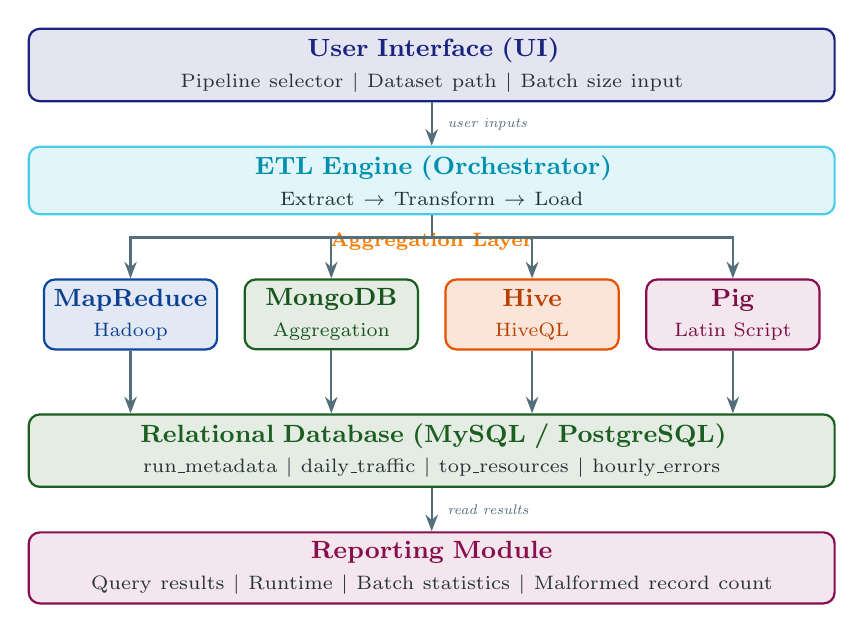
\begin{tikzpicture}[
  node distance = 0.6cm and 0.5cm,
  every node/.style = {font=\small},
  block/.style = {
    rectangle, rounded corners=4pt, 
    minimum width=2.8cm, minimum height=0.85cm,
    align=center, % <--- Changed from 'text centered' to fix the \\ error
    draw, thick
  },
  uiblock/.style   = {block, fill=PrimaryBlue!12, draw=PrimaryBlue, text width=10cm},
  etlblock/.style  = {block, fill=AccentCyan!12, draw=AccentCyan!70, text width=10cm},
  dbblock/.style   = {block, fill=SuccessGreen!12, draw=SuccessGreen, text width=10cm},
  repblock/.style  = {block, fill=PigPink!10, draw=PigPink, text width=10cm},
  arr/.style       = {-{Stealth[length=6pt]}, thick, color=MidGray},
  lbl/.style       = {font=\tiny\itshape, color=MidGray},
]

% UI Node
\node[uiblock] (ui) {%
  \textbf{\color{PrimaryBlue}User Interface (UI)}\\
  \scriptsize\color{DarkGray} Pipeline selector $|$ Dataset path $|$ Batch size input
};

% ETL Node
\node[etlblock, below=0.55cm of ui] (etl) {%
  \textbf{\color{AccentCyan!80!black}ETL Engine (Orchestrator)}\\
  \scriptsize\color{DarkGray} Extract $\rightarrow$ Transform $\rightarrow$ Load
};

% Pipeline row
\node[block, fill=MRBlue!12, draw=MRBlue, text=MRBlue!90!black,
      minimum width=2.2cm, below=0.8cm of etl, xshift=-3.825cm] (mr)
      {\textbf{MapReduce}\\\scriptsize Hadoop};
      
\node[block, fill=MongoGreen!12, draw=MongoGreen, text=MongoGreen!90!black,
      minimum width=2.2cm, below=0.8cm of etl, xshift=-1.275cm] (mg)
      {\textbf{MongoDB}\\\scriptsize Aggregation};
      
\node[block, fill=HiveYellow!15, draw=HiveYellow, text=HiveYellow!80!black,
      minimum width=2.2cm, below=0.8cm of etl, xshift=1.275cm] (hive)
      {\textbf{Hive}\\\scriptsize HiveQL};
      
\node[block, fill=PigPink!10, draw=PigPink, text=PigPink!90!black,
      minimum width=2.2cm, below=0.8cm of etl, xshift=3.825cm] (pig)
      {\textbf{Pig}\\\scriptsize Latin Script};

% Aggregation label - Fixed the color/font error here
\node[text=AccentOrange, font=\scriptsize\bfseries, below=0.1cm of etl]
      {Aggregation Layer};

% DB Node
\node[dbblock, below=0.8cm of mg, xshift=1.275cm] (db) {%
  \textbf{\color{SuccessGreen}Relational Database (MySQL / PostgreSQL)}\\
  \scriptsize\color{DarkGray} run\_metadata $|$ daily\_traffic $|$ top\_resources $|$ hourly\_errors
};

% Reporting Node
\node[repblock, below=0.55cm of db] (rep) {%
  \textbf{\color{PigPink}Reporting Module}\\
  \scriptsize\color{DarkGray} Query results $|$ Runtime $|$ Batch statistics $|$ Malformed record count
};

% Arrows
\draw[arr] (ui) -- (etl) node[lbl, midway, right=2pt] {user inputs};
\draw[arr] (etl.south) -- ++(0,-0.28) -| (mr.north);
\draw[arr] (etl.south) -- ++(0,-0.28) -| (mg.north);
\draw[arr] (etl.south) -- ++(0,-0.28) -| (hive.north);
\draw[arr] (etl.south) -- ++(0,-0.28) -| (pig.north);
\draw[arr] (mr.south) -- (db.north -| mr.south);
\draw[arr] (mg.south) -- (db.north -| mg.south);
\draw[arr] (hive.south) -- (db.north -| hive.south);
\draw[arr] (pig.south) -- (db.north -| pig.south);
\draw[arr] (db) -- (rep) node[lbl, midway, right=2pt] {read results};

\end{tikzpicture}
\caption{System architecture: the unified framework from UI through to the Reporting Module}
\label{fig:arch}
\end{figure}

\subsection{Component Overview}

The system comprises five tightly coupled components:

\vspace{4pt}
\begin{center}
\renewcommand{\arraystretch}{1.45}
\begin{tabular}{@{} >{}p{3.6cm} p{10.3cm} @{}}
\arrayrulecolor{PrimaryBlue!30}\toprule
\rowcolor{PrimaryBlue} \textcolor{white}{\textbf{Component}} & \textcolor{white}{\textbf{Responsibility}} \\
\midrule
\rowcolor{RowAlt}\textbf{\color{PrimaryBlue}User Interface (UI)} &
  Accepts pipeline selection (one of four systems), dataset path, and batch size. Triggers the ETL engine and passes control to the Reporting Module on completion. \\[2pt]
\textbf{\color{PrimaryBlue}ETL Engine} &
  Orchestrates Extract--Transform--Load. Reads raw logs, invokes the chosen service for parsing and aggregation, and pushes results to the relational database. \\[2pt]
\rowcolor{RowAlt}\textbf{\color{PrimaryBlue}Aggregation Layer} &
  The backend-specific execution layer (MapReduce / MongoDB / Hive / Pig) that computes the three mandatory queries over the structured records. \\[2pt]
\textbf{\color{PrimaryBlue}Relational Database} &
  PostgreSQL store holding all query results. Acts as the single source of truth for cross-pipeline comparison. \\[2pt]
\rowcolor{RowAlt}\textbf{\color{PrimaryBlue}Reporting Module} &
  Reads the relational database and presents results in structured format. \\
\arrayrulecolor{PrimaryBlue!30}\bottomrule
\end{tabular}
\end{center}

\section{User Interface Design}

The UI is a command-line or lightweight web front-end that presents the operator with pipeline and dataset configurations before any computation begins. The user can select the target pipeline and choose between two data input modes:

\begin{itemize}
  \item \textbf{Pre-split Dataset:} The user selects from a predefined list of dataset names that have already been partitioned into batches.
  \item \textbf{Custom Configuration:} The user manually specifies the path to a raw dataset file and the desired batch size. Upon execution, the system will dynamically split the file into batches before processing.
\end{itemize}

\vspace{6pt}
\begin{center}
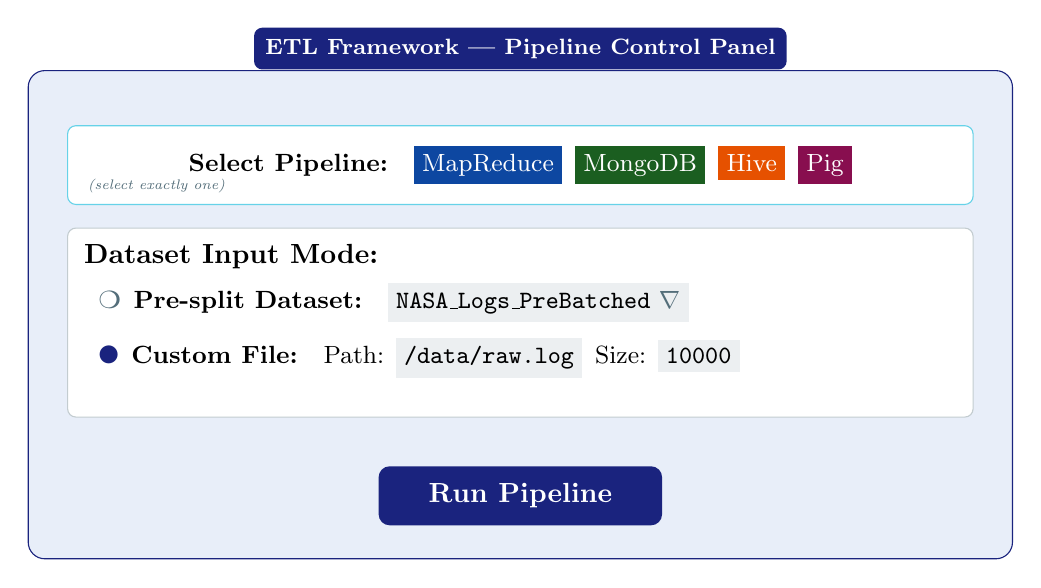
\begin{tikzpicture}[font=\small]
  \node[draw=PrimaryBlue, rounded corners=6pt, fill=LightBg,
        minimum width=12.5cm, minimum height=6.2cm] (panel) {};
  \node[above=0pt of panel.north, anchor=south,
        fill=PrimaryBlue, text=white, rounded corners=3pt,
        inner sep=4pt, font=\bfseries\footnotesize]
    {ETL Framework --- Pipeline Control Panel};

  % Pipeline selector row
  \node[draw=AccentCyan!60, rounded corners=3pt, fill=white, minimum width=11.5cm,
        minimum height=1.0cm, yshift=1.9cm] (ps) {%
    \textbf{Select Pipeline:}\quad
    \colorbox{MRBlue}{\textcolor{white}{\small MapReduce}}\enspace
    \colorbox{MongoGreen}{\textcolor{white}{\small MongoDB}}\enspace
    \colorbox{HiveYellow}{\textcolor{white}{\small Hive}}\enspace
    \colorbox{PigPink}{\textcolor{white}{\small Pig}}%
  };
  \node[font=\tiny\itshape\color{MidGray}, above=1pt of ps.south west, anchor=south west,
        xshift=4pt]{(select exactly one)};

  % Dataset Selection Box
  \node[draw=MidGray!35, rounded corners=3pt, fill=white, minimum width=11.5cm,
        minimum height=2.4cm, yshift=-0.1cm] (ds) {};
  \node[anchor=north west, font=\bfseries, inner sep=6pt] at (ds.north west) {Dataset Input Mode:};

  % Option 1: Pre-split
  \node[anchor=west] at ([xshift=8pt, yshift=0.25cm]ds.west) {%
    \textcolor{MidGray}{\ding{109}}\enspace\textbf{Pre-split Dataset:}\quad
    \colorbox{SoftGray}{\texttt{NASA\_Logs\_PreBatched} \textcolor{MidGray}{$\nabla$}}
  };
  
  % Option 2: Custom
  \node[anchor=west] at ([xshift=8pt, yshift=-0.45cm]ds.west) {%
    \textcolor{PrimaryBlue}{\ding{108}}\enspace\textbf{Custom File:}\quad
    Path: \colorbox{SoftGray}{\texttt{/data/raw.log}}\enspace
    Size: \colorbox{SoftGray}{\texttt{10000}}
  };

  % Run button
  \node[fill=PrimaryBlue, text=white, rounded corners=4pt,
        minimum width=3.6cm, minimum height=0.75cm, yshift=-2.3cm,
        font=\bfseries]
    {Run Pipeline};
\end{tikzpicture}
\end{center}

\vspace{4pt}
After execution, the UI passes control to the Reporting Module, which reads the relational database and renders structured results including query output tables, wall-clock runtime, batch statistics, and the malformed-record count.

\subsection{Reporting Module}

The Reporting Module reads from the relational database and presents:
\begin{itemize}
  \item \textbf{Run metadata:} pipeline name, run ID, batch ID, batch size, total runtime (seconds), malformed count
  \item \textbf{Query 1 table} --- Daily Traffic Summary (grouped by date and status code)
  \item \textbf{Query 2 table} --- Top 20 Requested Resources
  \item \textbf{Query 3 table} --- Hourly Error Analysis (grouped by date and hour)
\end{itemize}

\begin{notebox}
The framework is a single coherent tool. The execution backend is a pluggable module; all other components (UI, orchestration, database schema, reporting) remain identical across all four pipelines.
\end{notebox}

% ══════════════════════════════════════════════════════════════════════════════
%  SECTION 3 — BATCHING
% ══════════════════════════════════════════════════════════════════════════════
\section{Batching}
\subsection{Definition}

\begin{tcolorbox}[basebox, colback=LightBg, colframe=AccentCyan,
                  title={Batch Definition}]
\textbf{Batch} = a fixed number of input log records processed together in one execution unit.

\begin{itemize}
  \item \textbf{Batch size} --- configurable integer supplied via the UI (e.g.\ 10\,000 records).
  \item \textbf{Batch ID} --- sequential integer, incrementing by 1 from 1, for each subsequent batch.
  % \item \textbf{Final batch} --- if the last group contains fewer records than the configured batch size, it is still counted as a valid batch and given the next sequential ID.
\end{itemize}
\end{tcolorbox}

The \textbf{average batch size} is reported as:
\[
  {\text{batch size}} \;=\;
  \frac{\text{total records processed}}{\text{number of non-empty batches}}
\]

\subsection{Batch Processing Diagram}
Before records undergo parsing and aggregation, the framework orchestrates batching as dictated by the \texttt{PipelineRunner.java} driver. The system partitions the dataset based on the configured number of records per batch, and processes the queries sequentially.

\begin{figure}[H]
\centering
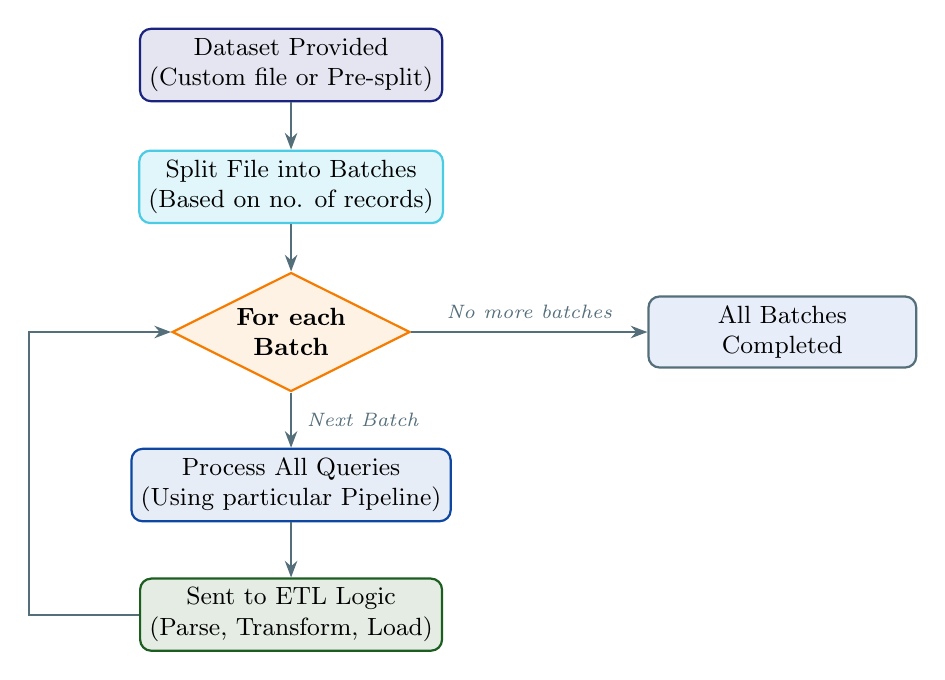
\begin{tikzpicture}[
  node distance=0.6cm and 0.8cm,
  every node/.style={font=\small},
  box/.style={rectangle, rounded corners=4pt, draw, thick, align=center,
              minimum width=3.4cm, minimum height=0.8cm},
  decision/.style={diamond, aspect=2, draw=AccentOrange, thick, fill=AccentOrange!10,
                   align=center, font=\small\bfseries, inner sep=2pt},
  arr/.style={-{Stealth[length=6pt]}, thick, color=MidGray},
  lbl/.style={font=\scriptsize\itshape, color=MidGray}
]

% Nodes
\node[box, fill=PrimaryBlue!12, draw=PrimaryBlue] (start) {Dataset Provided\\(Custom file or Pre-split)};

\node[box, fill=AccentCyan!12, draw=AccentCyan!70, below=0.6cm of start] (split) {Split File into Batches\\(Based on no. of records)};

\node[decision, below=0.6cm of split] (loop) {For each\\Batch};

\node[box, fill=LightBg, draw=MidGray, right=3cm of loop] (end) {All Batches\\Completed};

\node[box, fill=MRBlue!10, draw=MRBlue, below=0.7cm of loop] (queries) {Process All Queries\\(Using particular Pipeline)};

\node[box, fill=SuccessGreen!12, draw=SuccessGreen, below=0.7cm of queries] (etl) {Sent to ETL Logic\\(Parse, Transform, Load)};

% Arrows
\draw[arr] (start) -- (split);
\draw[arr] (split) -- (loop);
\draw[arr] (loop) -- node[lbl, right=2pt] {Next Batch} (queries);
\draw[arr] (loop) -- node[lbl, above=1pt] {No more batches} (end);
\draw[arr] (queries) -- (etl);

% Back edge for loop
\draw[arr] (etl.west) -- ++(-1.4,0) |- (loop.west);

\end{tikzpicture}
\caption{Flow chart showing dataset splitting and query execution per batch.}
\label{fig:batching_flow}
\end{figure}

% ══════════════════════════════════════════════════════════════════════════════
%  SECTION 4 — PARSING STRATEGY
% ══════════════════════════════════════════════════════════════════════════════
\section{Parsing Strategy}
\label{sec:parsing}

\subsection{Log Format}

Each line in the NASA HTTP log follows the Combined Log Format. A representative record is:

\begin{tcolorbox}[basebox, 
                  % left=5pt, right=5pt, % Tighten padding to gain horizontal space
                  colback=DarkGray!90, colframe=DarkGray,
                  fontupper=\ttfamily\footnotesize\color{white}] % Reduced from \small to \footnotesize
199.72.81.55 - - [01/Jul/1995:00:00:01 -0400] "GET /history/apollo/ HTTP/1.0" 200 6245
\end{tcolorbox}

\subsection{Extracted Fields}
\vspace{4pt}
\begin{center}
\renewcommand{\arraystretch}{1.35}
\begin{tabular}{@{} >{\ttfamily\small}l >{\small}l >{\small\itshape}l @{}}
\toprule
\textnormal{\textbf{Raw value}} & \textbf{Extracted field} & \textbf{Notes} \\
\midrule
199.72.81.55              & host             & IP address or hostname \\
01/Jul/1995:00:00:01 -0400 & timestamp        & Full timestamp string \\
01/Jul/1995               & log\_date        & Date portion extracted from timestamp \\
00                        & log\_hour        & Hour portion (0--23) \\
GET                       & http\_method     & HTTP Method \\
/history/apollo/          & resource\_path   & Target URL path requested by the client. \\
HTTP/1.0                  & protocol\_version & HTTP version protocol string. \\
200                       & status\_code     & Integer HTTP reply code \\
6245                      & bytes\_transferred & Integer; \texttt{-} is treated as 0 \\
\bottomrule
\end{tabular}
\end{center}

\subsection{Regex-Based Parsing}

A robust master regular expression (\texttt{java.util.regex.Pattern}) captures all eight required fields in one pass. Instead of capturing the entire timestamp string, targeted capture groups selectively extract the \texttt{logDate} and \texttt{logHour} directly. The \texttt{bytes} capture group enforces strict pattern validation by only matching digits or a hyphen.

\begin{lstlisting}[style=regexstyle, caption={Master regular expression for log-line parsing}]
^(\S+)\s+\S+\s+\S+\s+\[(\d{2}/\w{3}/\d{4}):(\d{2}):\d{2}:\d{2}\s+[+-]\d{4}\]\s+"([A-Z]+)\s+(\S+)\s+(HTTP/[\d.]+)"\s+(\d{3})\s+(\d+|-)$
\end{lstlisting}

Capture-group mapping:
\texttt{(1)~host}, \texttt{(2)~logDate}, \texttt{(3)~logHour}, \texttt{(4)~method},
\texttt{(5)~resource}, \texttt{(6)~protocol}, \texttt{(7)~statusCode},
\texttt{(8)~bytes\_raw}.

The \texttt{bytes} field is derived as:
\[
  \text{bytes} =
  \begin{cases}
    0 & \text{if } \texttt{bytes\_raw} = \texttt{"-"} \\
    \text{int}(\texttt{bytes\_raw}) & \text{otherwise}
  \end{cases}
\]

\subsection{Parsing Constraints}

\begin{constraintbox}
\begin{itemize}
  \item If the bytes field contains \texttt{-}, it \textbf{must} be substituted with \textbf{0} (not discarded).
  \item Malformed records (lines that do not match the master regex) must \textbf{not} be silently dropped. A \texttt{malformed\_record\_counter} is incremented and the count is persisted to the metadata table at the end of each run.
\end{itemize}
\end{constraintbox}

\subsection{Parsing Flow Diagram}

\begin{figure}[H]
\centering
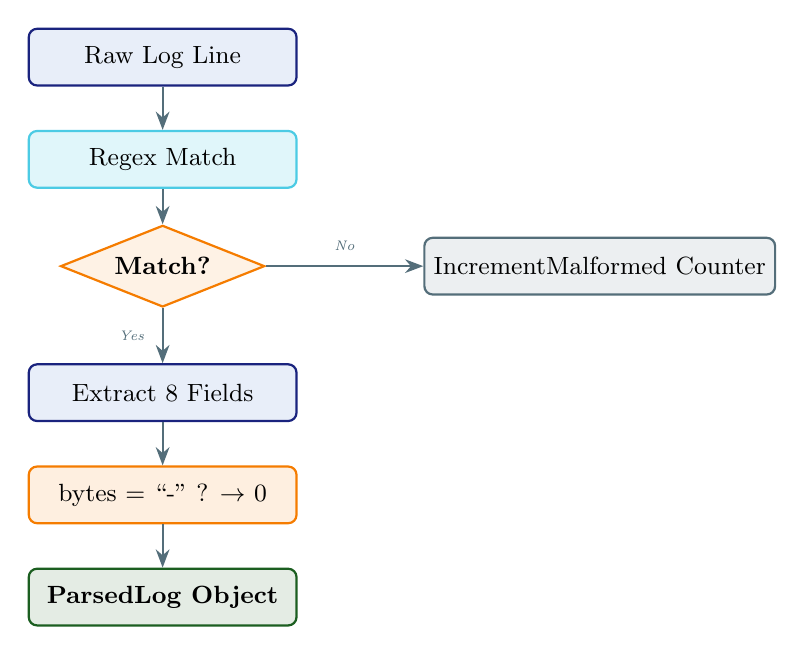
\begin{tikzpicture}[
  node distance=0.55cm,
  box/.style={rectangle, rounded corners=3pt, draw, thick, minimum width=3.4cm,
              minimum height=0.72cm, text centered, font=\small},
  decision/.style={diamond, draw=AccentOrange, thick, fill=AccentOrange!10,
                   aspect=2.5, minimum height=0.8cm,
                   text centered, font=\small\bfseries},
  arr/.style={-{Stealth}, thick, MidGray},
  lbl/.style={font=\tiny\itshape, MidGray},
]

\node[box, fill=LightBg, draw=PrimaryBlue] (raw) {Raw Log Line};
\node[box, fill=AccentCyan!12, draw=AccentCyan!70, below=of raw] (regex) {Regex Match};
\node[decision, below=0.45cm of regex] (match) {Match?};
\node[box, fill=SoftGray, draw=MidGray, right=2cm of match] (bad)
  {Increment\\Malformed Counter};
\node[box, fill=LightBg, draw=PrimaryBlue, below=0.7cm of match] (fields)
  {Extract 8 Fields};
\node[box, fill=AccentOrange!12, draw=AccentOrange, below=of fields] (bytes)
  {bytes = ``-'' ? $\to$ 0};
\node[box, fill=SuccessGreen!12, draw=SuccessGreen, below=of bytes] (struct)
  {\textbf{ParsedLog Object}};

\draw[arr] (raw) -- (regex);
\draw[arr] (regex) -- (match);
\draw[arr] (match) -- node[lbl, left=3pt]{Yes} (fields);
\draw[arr] (match) -- node[lbl, above=2pt]{No} (bad);
\draw[arr] (fields) -- (bytes);
\draw[arr] (bytes) -- (struct);

\end{tikzpicture}
\caption{Parsing flow: from raw log line to validated ParsedLog object}
\label{fig:parse}
\end{figure}

% ══════════════════════════════════════════════════════════════════════════════
%  SECTION 5 — ETL WORKFLOW
% ══════════════════════════════════════════════════════════════════════════════
\section{ETL Workflow}

The ETL workflow remains logically identical across the implemented execution pipelines (MapReduce and MongoDB), ensuring consistent methodology regardless of the underlying engine.

\subsection{Three Phases}

\subsubsection{Extract}
\begin{itemize}
  \item Raw log files are read from the path supplied by the user through the UI. No preprocessing outside the chosen execution pipeline is permitted (no manual CSV conversion, JSON conversion, filtering, or editing). Files are read line by line and dispatched to the transform stage in configurable batches.
  \item The \texttt{PipelineRunner.java} supplies the dataset path and generates a unique SQL \texttt{runId} via \texttt{MetadataDAO.java}.
\end{itemize}

\subsubsection{Transform}
\begin{itemize}
  \item \textbf{Parsing:} The master regex ,i.e, \texttt{LogParser.java} regex validates and extracts the 8 core fields line-by-line.
  \item \textbf{Cleaning \& Tracking:} Hyphens (\texttt{-}) in bytes are safely converted to \texttt{0}. Malformed records dynamically increment a tracking counter and are excluded from calculations.
  \item \textbf{Query Aggregation:} The engine executes grouping and arithmetic logic (e.g., counting requests, summing bytes, distinct hosts).
\end{itemize}

\subsubsection{Load}
\begin{itemize}
  \item \textbf{Result Retrieval:} The three mandatory queries are executed on the structured data within the chosen backend.
  \item \textbf{Database Insertion:} Structured results are persisted directly to PostgreSQL via Data Access Objects .
  \item \textbf{Finalization:} Run metadata (runtime, malformed count, batch statistics) is inserted into the \texttt{run\_metadata} table.
\end{itemize}

\subsection{ETL Flow Diagram}

\begin{figure}[H]
\centering
% \resizebox{\textwidth}{!} ensures the diagram fits your page width perfectly
\resizebox{\textwidth}{!}{
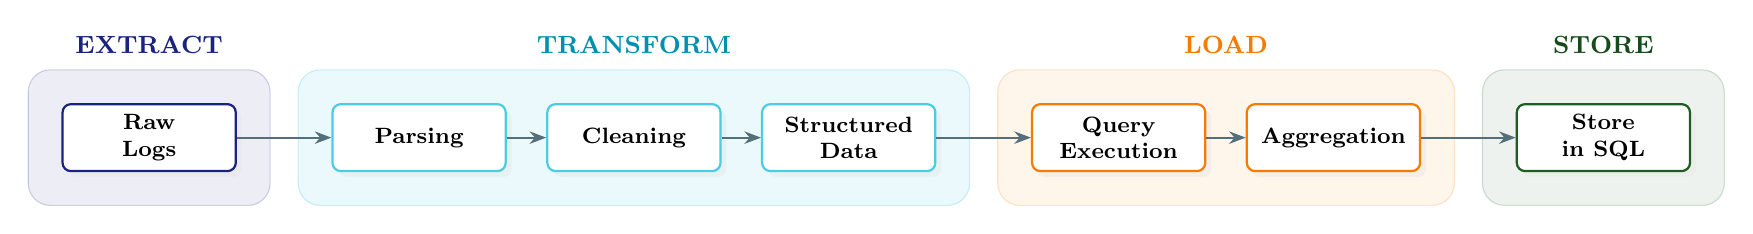
\begin{tikzpicture}[
    node distance = 0.5cm and 0.4cm,
    % Style for the individual process blocks
    stage/.style = {
        rectangle, rounded corners=3pt, draw, thick,
        minimum width=2.2cm, minimum height=0.85cm,
        align=center, font=\footnotesize\bfseries, 
        fill=white, drop shadow={fill=black!10, opacity=0.4}
    },
    % Style for the shaded phase backgrounds
    phase/.style = {
        rounded corners=8pt, inner sep=12pt, 
        draw opacity=0.2, fill opacity=0.08
    },
    % Style for phase labels
    label/.style = {font=\small\bfseries, yshift=2pt},
    arr/.style = {-{Stealth[length=6pt]}, thick, color=MidGray},
]

% --- 1. DEFINE NODES ---

% EXTRACT Phase
\node[stage, draw=PrimaryBlue] (raw) {Raw\\Logs};

% TRANSFORM Phase
\node[stage, draw=AccentCyan!70, right=1.2cm of raw] (parse) {Parsing};
\node[stage, draw=AccentCyan!70, right=0.5cm of parse] (clean) {Cleaning};
\node[stage, draw=AccentCyan!70, right=0.5cm of clean] (struct) {Structured\\Data};

% LOAD Phase
\node[stage, draw=AccentOrange, right=1.2cm of struct] (query) {Query\\Execution};
\node[stage, draw=AccentOrange, right=0.5cm of query] (agg) {Aggregation};

% STORE Phase
\node[stage, draw=SuccessGreen, right=1.2cm of agg] (db) {Store\\in SQL};


% --- 2. CREATE BACKGROUND BOXES & LABELS ---
\begin{scope}[on background layer]
    % Extract Container
    \node[phase, fill=PrimaryBlue, draw=PrimaryBlue, fit=(raw)] (bg_ext) {};
    \node[label, color=PrimaryBlue, above=0pt of bg_ext] {EXTRACT};

    % Transform Container
    \node[phase, fill=AccentCyan, draw=AccentCyan, fit=(parse)(struct)] (bg_trans) {};
    \node[label, color=AccentCyan!80!black, above=0pt of bg_trans] {TRANSFORM};

    % Load Container
    \node[phase, fill=AccentOrange, draw=AccentOrange, fit=(query)(agg)] (bg_load) {};
    \node[label, color=AccentOrange, above=0pt of bg_load] {LOAD};

    % Store Container
    \node[phase, fill=SuccessGreen, draw=SuccessGreen, fit=(db)] (bg_store) {};
    \node[label, color=SuccessGreen!80!black, above=0pt of bg_store] {STORE};
\end{scope}


% --- 3. DRAW CONNECTORS ---
\draw[arr] (raw) -- (parse);
\draw[arr] (parse) -- (clean);
\draw[arr] (clean) -- (struct);
\draw[arr] (struct) -- (query);
\draw[arr] (query) -- (agg);
\draw[arr] (agg) -- (db);

\end{tikzpicture}
}
\caption{The unified ETL Workflow: consistent processing across all four pipelines.}
\label{fig:refined_etl}
\end{figure}

\begin{notebox}
The parsing rules, cleaning rules, field definitions, query definitions, and output schema are strictly identical across MapReduce, MongoDB, Hive, and Pig. This ensures cross-pipeline comparisons are fair and meaningful.
\end{notebox}
% ══════════════════════════════════════════════════════════════════════════════
%  SECTION 4 — PIPELINE OVERVIEW
% ══════════════════════════════════════════════════════════════════════════════
\section{Pipeline Overview}

Each pipeline executes the same three analytical queries using a different processing paradigm. All four implement equivalent semantics: the same parsing rules, cleaning rules, filtering conditions, grouping logic, and aggregation definitions.

\begin{mrbox}
\textbf{Paradigm:} Low-level, programmer-controlled parallel computation on HDFS.

\textbf{Execution model:} Custom Mapper and Reducer classes. The Mapper applies the master regex to each log line and emits typed key--value pairs. The Reducer aggregates values per key (e.g., summing bytes, counting requests, collecting distinct hosts).

\textbf{Characteristics:} Fine-grained control over the map phase, shuffle/sort, and reduce phase. Hadoop's \texttt{InputSplit} mechanism naturally partitions data into processing chunks that correspond to logical batches.

\textbf{Query implementation:} Each of the three queries is a separate MapReduce job. Jobs are chained by the orchestrator, and results are loaded to SQL at the end of each chain.
\end{mrbox}

\vspace{5pt}

\begin{mongobox}
\textbf{Paradigm:} Document-oriented NoSQL with a declarative aggregation framework.

\textbf{Execution model:} Parsed log records are inserted as BSON documents into a collection. Queries are expressed using the MongoDB Aggregation Pipeline: \texttt{\$match} for filtering, \texttt{\$group} for aggregation, \texttt{\$sort} and \texttt{\$limit} for top-$N$ ranking.

\textbf{Characteristics:} Schema-flexible; easy to express the three queries in a concise, declarative style. Data is inserted in configurable-size chunks (batches) tracked by batch ID.
\end{mongobox}

\vspace{5pt}

\begin{hivebox}
\textbf{Paradigm:} SQL-like query language (HiveQL) over Hadoop.

\textbf{Execution model:} The log file is loaded into an external Hive table backed by the raw text. Queries are written as standard \texttt{SELECT ... GROUP BY ...} HiveQL statements. Hive compiles these internally into MapReduce or Tez jobs.

\textbf{Characteristics:} The three mandatory queries map almost directly to SQL, making Hive the most concise implementation. Partitioning or chunk-based loading is used to emulate batching.
\end{hivebox}

\vspace{5pt}

\begin{pigbox}
\textbf{Paradigm:} Dataflow scripting language (Pig Latin) that compiles to MapReduce.

\textbf{Execution model:} A Pig Latin script loads the data, applies a custom UDF or regex-based \texttt{LOAD} function for parsing, then uses \texttt{FILTER}, \texttt{GROUP}, and \texttt{FOREACH ... GENERATE} to compute the required aggregations.

\textbf{Characteristics:} Step-by-step, explicit transformation pipeline. Each data transformation is visible as a named Pig relation, making the logic easy to audit and debug.
\end{pigbox}

% ══════════════════════════════════════════════════════════════════════════════
%  SECTION 5 — BATCHING APPROACH
% ══════════════════════════════════════════════════════════════════════════════
\section{Batching Approach}

\subsection{Definition}

\begin{tcolorbox}[basebox, colback=LightBg, colframe=AccentCyan,
                  title={Batch Definition}]
\textbf{Batch} = a fixed number of input log records processed together in one execution unit.

\begin{itemize}
  \item \textbf{Batch size} --- configurable integer supplied by the user via the UI (e.g.\ 10\,000 records).
  \item \textbf{Batch ID} --- sequential integer starting from \textbf{1}, incrementing by 1 for each subsequent batch.
  \item \textbf{Final batch} --- if the last group contains fewer records than the configured batch size, it is still counted as a valid batch and given the next sequential ID.
\end{itemize}
\end{tcolorbox}

The \textbf{average batch size} is reported as:
\[
  \overline{\text{batch size}} \;=\;
  \frac{\text{total records processed}}{\text{number of non-empty batches}}
\]

\subsection{Pipeline-Specific Batching}

\begin{center}
\renewcommand{\arraystretch}{1.4}
\begin{tabularx}{\linewidth}{@{} >{\bfseries\small}l X @{}}
\toprule
Pipeline & Batching mechanism \\
\midrule
MapReduce &
  Hadoop's \texttt{NLineInputFormat} is configured so that each InputSplit contains exactly \emph{N} lines, where \emph{N} equals the chosen batch size. Each InputSplit is processed by one Mapper, constituting one logical batch. \\[3pt]
MongoDB &
  Parsed records are inserted via \texttt{insert\_many()} in Python list chunks of size $= $ batch size. Each \texttt{insert\_many()} call represents one batch; \texttt{batch\_id} is tracked and stored per chunk in the metadata table. \\[3pt]
Hive &
  The orchestrator splits the raw log file into chunk files, each containing exactly \emph{batch\_size} lines. Chunk files are loaded sequentially into the Hive table, and each load operation is assigned a sequential \texttt{batch\_id}. \\[3pt]
Pig &
  Pre-split chunk files (produced by the orchestrator) are passed to Pig runs sequentially. Each Pig execution processes one chunk, corresponding to one batch. \\
\bottomrule
\end{tabularx}
\end{center}

\subsection{Batch Processing Diagram}

\begin{figure}[H]
\centering
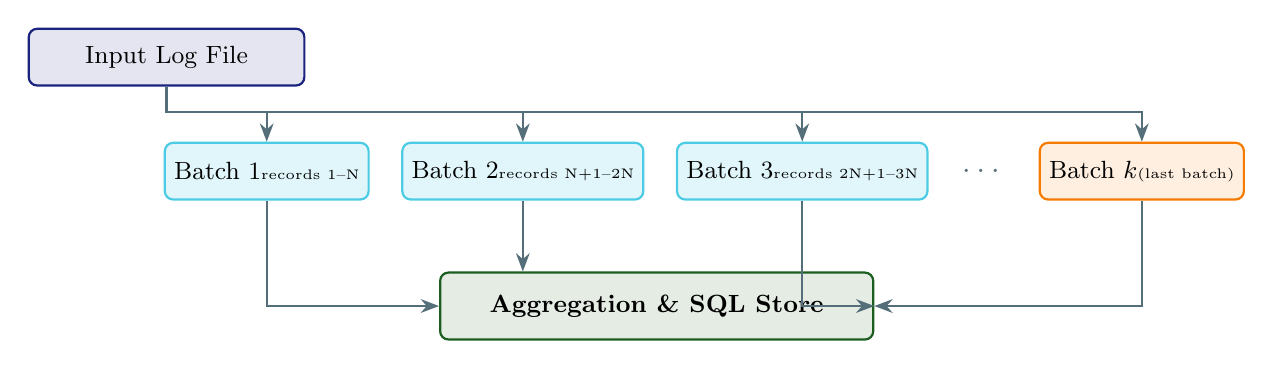
\begin{tikzpicture}[
  node distance=0.5cm and 0.5cm,
  box/.style={rectangle, rounded corners=3pt, draw, thick,
              minimum width=2.3cm, minimum height=0.72cm,
              text centered, font=\small},
  arr/.style={-{Stealth}, thick, MidGray},
]

\node[box, fill=PrimaryBlue!12, draw=PrimaryBlue, minimum width=3.5cm] (input)
  {Input Log File};

\node[box, fill=AccentCyan!12, draw=AccentCyan!70,
      below right=0.7cm and -1.8cm of input] (b1)
  {Batch 1\\{\tiny records 1--N}};
\node[box, fill=AccentCyan!12, draw=AccentCyan!70,
      right=0.4cm of b1] (b2)
  {Batch 2\\{\tiny records N+1--2N}};
\node[box, fill=AccentCyan!12, draw=AccentCyan!70,
      right=0.4cm of b2] (b3)
  {Batch 3\\{\tiny records 2N+1--3N}};
\node[font=\large\color{MidGray}, right=0.3cm of b3] (dots) {\ldots};
\node[box, fill=AccentOrange!12, draw=AccentOrange,
      right=0.3cm of dots] (bn)
  {Batch $k$\\{\tiny (last batch)}};

\node[box, fill=SuccessGreen!12, draw=SuccessGreen,
      below=0.9cm of b2, xshift=1.7cm, minimum width=5.5cm,
      minimum height=0.85cm] (agg)
  {\textbf{Aggregation \& SQL Store}};

\draw[arr] (input.south) -- ++(0,-0.32) -| (b1.north);
\draw[arr] (input.south) -- ++(0,-0.32) -| (b2.north);
\draw[arr] (input.south) -- ++(0,-0.32) -| (b3.north);
\draw[arr] (input.south) -- ++(0,-0.32) -| (bn.north);

\draw[arr] (b1.south) |- (agg.west);
\draw[arr] (b2.south) -- (agg.north -| b2.south);
\draw[arr] (b3.south) |- (agg);
\draw[arr] (bn.south) |- (agg.east);

\end{tikzpicture}
\caption{Batch processing: input is partitioned into $k$ equal batches; the final batch may contain fewer than $N$ records}
\label{fig:batch}
\end{figure}

% ══════════════════════════════════════════════════════════════════════════════
%  SECTION 6 — RELATIONAL DATABASE SCHEMA
% ══════════════════════════════════════════════════════════════════════════════
\section{Relational Database Schema}

\subsection{Design Rationale}

The schema separates run-level metadata from query results. One metadata table stores information common to all queries (pipeline name, runtime, batch info). Three result tables---one per mandatory query---hold the aggregated outputs and reference the metadata table via \texttt{run\_id} (foreign key). This design allows any run's results to be retrieved, filtered by pipeline or batch, and compared against other runs.

\subsection{Metadata Table: \texttt{run\_metadata}}

\begin{schematable}
\begin{tabularx}{\linewidth}{@{} >{\ttfamily\small}l >{\small}l X @{}}
\toprule
\textnormal{\textbf{Column}} & \textbf{Type} & \textbf{Description} \\
\midrule
run\_id              & SERIAL PK    & Auto-incremented unique identifier for each run \\
pipeline\_name       & VARCHAR(20)  & One of: \texttt{mapreduce}, \texttt{mongodb}, \texttt{hive}, \texttt{pig} \\
batch\_id            & INTEGER      & Sequential batch identifier (starts at 1) \\
batch\_size          & INTEGER      & Configured number of records per batch \\
runtime              & FLOAT        & Wall-clock time in seconds (ETL only; excludes report time) \\
malformed\_record\_count & INTEGER  & Number of log lines that failed regex parsing \\
timestamp            & TIMESTAMP    & UTC datetime when the run was recorded \\
\bottomrule
\end{tabularx}
\end{schematable}

\subsection{Result Table 1: \texttt{daily\_traffic}}

Stores the output of Query 1 (Daily Traffic Summary).

\begin{schematable}
\begin{tabularx}{\linewidth}{@{} >{\ttfamily\small}l >{\small}l X @{}}
\toprule
\textnormal{\textbf{Column}} & \textbf{Type} & \textbf{Description} \\
\midrule
id            & SERIAL PK  & Row identifier \\
run\_id       & INTEGER FK & References \texttt{run\_metadata.run\_id} \\
log\_date     & DATE       & Date of the log entries (e.g.\ 01/Jul/1995) \\
status\_code  & INTEGER    & HTTP reply code \\
request\_count & BIGINT    & Total number of requests for this date--code pair \\
total\_bytes  & BIGINT     & Sum of bytes transferred for this date--code pair \\
\bottomrule
\end{tabularx}
\end{schematable}

\subsection{Result Table 2: \texttt{top\_resources}}

Stores the output of Query 2 (Top Requested Resources). Only the top 20 rows by request count are stored per run.

\begin{schematable}
\begin{tabularx}{\linewidth}{@{} >{\ttfamily\small}l >{\small}l X @{}}
\toprule
\textnormal{\textbf{Column}} & \textbf{Type} & \textbf{Description} \\
\midrule
id                 & SERIAL PK  & Row identifier \\
run\_id            & INTEGER FK & References \texttt{run\_metadata.run\_id} \\
resource\_path     & TEXT       & Requested URL path \\
request\_count     & BIGINT     & Number of times this resource was requested \\
total\_bytes       & BIGINT     & Total bytes served for this resource \\
distinct\_host\_count & BIGINT  & Number of unique hosts requesting this resource \\
\bottomrule
\end{tabularx}
\end{schematable}

\subsection{Result Table 3: \texttt{hourly\_errors}}

Stores the output of Query 3 (Hourly Error Analysis).

\begin{schematable}
\begin{tabularx}{\linewidth}{@{} >{\ttfamily\small}l >{\small}l X @{}}
\toprule
\textnormal{\textbf{Column}} & \textbf{Type} & \textbf{Description} \\
\midrule
id                    & SERIAL PK  & Row identifier \\
run\_id               & INTEGER FK & References \texttt{run\_metadata.run\_id} \\
log\_date             & DATE       & Date of the log entries \\
log\_hour             & SMALLINT   & Hour of day (0--23) \\
error\_request\_count  & BIGINT     & Requests with status code 400--599 \\
total\_request\_count  & BIGINT     & All requests in this date--hour slot \\
error\_rate           & FLOAT      & \texttt{error\_request\_count / total\_request\_count} \\
distinct\_error\_hosts & BIGINT     & Unique hosts generating error responses \\
\bottomrule
\end{tabularx}
\end{schematable}

% ══════════════════════════════════════════════════════════════════════════════
%  SECTION 7 — EQUIVALENCE ACROSS PIPELINES
% ══════════════════════════════════════════════════════════════════════════════
\section{Ensuring Equivalence Across Pipelines}

To make the cross-pipeline comparison fair and meaningful, the following invariants are enforced throughout the implementation:

\begin{enumerate}
  \item \textbf{Same dataset.} All pipelines read the identical NASA HTTP log files downloaded from the official Internet Traffic Archive. No manual preprocessing, CSV conversion, JSON conversion, filtering, or editing is applied outside the selected pipeline.

  \item \textbf{Same parsing rules.} The master regex and field-extraction logic are defined once at the architecture level and translated faithfully into each backend (Mapper code, MongoDB UDF, Hive SerDe or regex UDF, Pig LOAD function with UDF).

  \item \textbf{Same query definitions.} The three mandatory queries specify exact output columns, filtering conditions (e.g.\ status 400--599 for errors), and aggregation semantics. These are not relaxed or simplified for any particular pipeline.

  \item \textbf{Same batch size.} In any comparative experiment, the same batch-size value is supplied to all four pipelines via the shared UI.

  \item \textbf{Same output schema.} All results are written to the shared relational database in an identical schema regardless of which backend produced them. This allows direct SQL comparison across runs.
\end{enumerate}

% ══════════════════════════════════════════════════════════════════════════════
%  SECTION 8 — DIAGRAM INDEX
% ══════════════════════════════════════════════════════════════════════════════
\section{Diagram Index}

\begin{center}
\renewcommand{\arraystretch}{1.45}
\begin{tabular}{@{} c >{\bfseries}l l @{}}
\arrayrulecolor{PrimaryBlue!30}\toprule
\rowcolor{PrimaryBlue}
  \textcolor{white}{\textbf{Figure}} & \textcolor{white}{\textbf{Section}} & \textcolor{white}{\textbf{Description}} \\
\midrule
\rowcolor{RowAlt}\ref{fig:arch}  & 1 & System Architecture --- UI through to Reporting Module \\
\ref{fig:parse} & 2 & Parsing Flow --- Raw line to validated structured record \\
\rowcolor{RowAlt}\ref{fig:etl}   & 3 & ETL Workflow --- Extract, Transform, Load \\
\ref{fig:batch} & 5 & Batch Processing --- Input split into $k$ equal batches \\
\arrayrulecolor{PrimaryBlue!30}\bottomrule
\end{tabular}
\end{center}

% ══════════════════════════════════════════════════════════════════════════════
%  SECTION 9 — PHASE 1 STATUS
% ══════════════════════════════════════════════════════════════════════════════
\section{Phase 1 Prototype Status}

At the time of this Phase 1 review, the following components are complete or in active development:

\begin{center}
\renewcommand{\arraystretch}{1.4}
\begin{tabular}{@{} l c c @{}}
\arrayrulecolor{PrimaryBlue!30}\toprule
\rowcolor{PrimaryBlue}
  \textcolor{white}{\textbf{Component}} & \textcolor{white}{\textbf{Status}} & \textcolor{white}{\textbf{Applies to}} \\
\midrule
\rowcolor{SuccessGreen!8}UI (pipeline selector, dataset path, batch size) & \textcolor{SuccessGreen}{\ding{52}\;Done} & All \\
\rowcolor{SuccessGreen!8}Master regex parser + malformed counter           & \textcolor{SuccessGreen}{\ding{52}\;Done} & All \\
\rowcolor{SuccessGreen!8}MapReduce ETL (Q1, Q2, Q3)                        & \textcolor{SuccessGreen}{\ding{52}\;Done} & MapReduce \\
\rowcolor{SuccessGreen!8}MongoDB ETL (Q1, Q2, Q3)                          & \textcolor{SuccessGreen}{\ding{52}\;Done} & MongoDB \\
\rowcolor{AccentOrange!10}Hive ETL                                          & \textcolor{AccentOrange}{\ding{115}\;In Progress} & Hive \\
\rowcolor{AccentOrange!10}Pig ETL                                           & \textcolor{AccentOrange}{\ding{115}\;In Progress} & Pig \\
\rowcolor{SuccessGreen!8}Relational database schema and load scripts        & \textcolor{SuccessGreen}{\ding{52}\;Done} & All \\
\rowcolor{SuccessGreen!8}Reporting module                                   & \textcolor{SuccessGreen}{\ding{52}\;Done} & All \\
\arrayrulecolor{PrimaryBlue!30}\bottomrule
\end{tabular}
\end{center}

Phase 2 will complete the Hive and Pig pipelines, execute comparative experiments across all four backends using the same batch size, and document runtime observations, implementation difficulty, and correctness comparisons.

\vspace{1.5cm}
\begin{center}
\begin{tcolorbox}[enhanced, arc=8pt, boxrule=0pt,
  colback=PrimaryBlue, colframe=PrimaryBlue,
  width=10cm, halign=center,
  drop shadow={fill=black!20, opacity=0.4}]
  \centering
  {\color{AccentCyan}\rule{6cm}{0.6pt}}\\[6pt]
  {\small\color{white}\itshape End of Phase 1 Report}\\[3pt]
  {\small\color{AccentCyan!80}\bfseries DAS 839 \;\textcolor{white}{||}\; NoSQL Systems}\\[6pt]
  {\color{AccentCyan}\rule{6cm}{0.6pt}}
\end{tcolorbox}
\end{center}

\end{document}